\chapter{Zabbix}

\textbf{Zabbix}, tal como o Nagios Core, é uma ferramenta de monitorização de sistemas de rede e informação \textit{open-source} \cite{Zabbix}.
Permite a supervisão de diversos sistemas tais como redes, servidores VMs e serviços de cloud.
Paralelamente a estes serviços, é também possível monitorizar o estado hardware em sistemas onde o Zabbix esteja instalado.
O Zabbix funciona com apoio de uma base de dados. 
Se por predefinição, o Nagios usa MySQL, o Zabbix permite escolher de uma gama de opções, nomeadamente MySQL, MariaDB, PostgreSQL, etc.

O Zabbix não funciona à base de plugins, mas sim de \textbf{items}.
Este items têm o mesmo princípio de funcionamento, consistindo em testes executados periodicamente para monitorizar uma característica específica.
Os items podem ter outputs diferentes, quer seja números, strings ou booleanos.

No entanto, é de notar que o Zabbix não sabe interpretar o output destes items como correto ou não.
Para se definir o estado de um serviço ou \textit{feature}, é preciso definir os \textbf{triggers}.

Triggers correspondem a testes que são feitos ao output dos items.
Por exemplo, se um determinado item tem como output possível \textbf{1/0},
um trigger pode definir 1 como OK e 0 como ERROR, dando desse modo feedback ao utilizar sobre o estado de serviço de uma forma mais direta.

Para simplificar o processo de setup, e evitar a configuração manual de todos os items e correspondentes triggers,
são fornecidos \textbf{Templates} que contêm um conjunto de items e triggers adequados para determinados contextos.
Por exemplo, o template \textbf{Template App HTTP Service} contém um item que testa um servidor HTTP, e um trigger que processa o output para determinar o seu estado.
Alguns templates também contêm \textbf{dashboards}, que são uma compilação visual de informação relevante naquele template.

\pagebreak

\section{Instalação e configuração}

A instalação foi feita de acordo com a documentação do Zabbix \cite{Zabbix_setup} no Tux13.

Similarmente ao Nagios, o Zabbix oferece duas opções de monitorização:

\begin{itemize}
    \item Zabbix-agent: O Zabbix-agent é instalado no host destino, onde este coleta informação relevante do funcionamento do sistema, como a carga de CPU, disco, etc.
    O servidor Zabbix recebe depois esta informação diretamente do host, podendo assim mostrar várias estatísticas locais. É adequado quando queremos monitorizar um servidor ou computador.
    \item \textit{Agentless}: Os testes são feitos apenas sobre serviços que possam ser acedidos externamente, por exemplo, um servidor HTTP.
    Não é preciso instalar nada, sendo que a monitorização destes sistemas recorre a protocolos de comunicação como HTTP, SSH, SNMP, TELNET, etc. É adequado quando queremos monitorizar um componente de \textit{networking}, como um Router ou Switch.
\end{itemize}

Tendo isto consideração, a abordagem \textbf{Zabbix-agent} foi utilizada nos casos dos Tuxs, e a abordagem \textbf{Agentless} no Switch e no Router.

O próximo passo consiste na instalação dos diferentes \textit{packages} requeridos pelo Zabbix.
É aqui que se define também qual é a base de dados que se vai usar. A escolhida foi a \textbf{PostgreSQL}.

Foram definidos \textit{Users} e as respetivas \textit{passwords} quer para o Zabbix, quer para a base de dados.
O passo seguinte consiste na criação da base de dados que contém todas as configurações do Zabbix \footnote{A documentação online está errada a vários níveis, quer nos diretórios, quer na estrutura da base de dados.
No entanto a documentação fornecida localmente após a instalação do respetivo \textit{package} está correta}.

Após a configuração inicial, é definido no ficheiro \verb|/etc/zabbix/zabbix_server.conf| os parâmetros da base de dados criada:

\begin{lstlisting}
    DBHost= (string nula para o caso do PostgreSQL)
    DBName=zabbix
    DBUser=zabbix
    DBPassword=12345
\end{lstlisting}

Posteriormente, é feita a configuração final na página Web do Zabbix.
Após este passo, é possível iniciar a configuração da monitorização da rede.

A instalação dos agentes no Tux12, Tux13 e Tux14 é feita com a instalação do devido \textit{package}.
Posteriormente, o ficheiro \verb|/etc/zabbix/zabbix_agentd.conf| é modificado, especificando-se nas linhas “Server=” and “ServerActive=” o IP do servidor Zabbix.
O agente no Tux13 também é instalado pois é necessário para se poder fazer a monitorização do hardware do sistema no servidor.

\pagebreak

Ao contrário do Nagios, o Zabbix não é configurado localmente no sistema editando ficheiros de configuração, mas sim na interface Web do software.
Logo à partida, é possível afirmar que, para o utilizador comum, é mais fácil usar uma UI do que recorrer extensivamente ao terminal.

Os \textbf{Hosts} são a primeira coisa a definir.
A definição de um host consiste na definição da interface de comunicação entre o host e o servidor.
Além do IP, é preciso definir se esses hosts tem ou não agente.
No caso do Tux12 e Tux14, foi definida uma interface com agente.
No caso do Switch e do Router, foi definida uma interface com recurso ao protocolo SNMP.

\begin{figure}[H]
    \centering
    \begin{subfigure}[b]{0.9\textwidth}
        \centering
        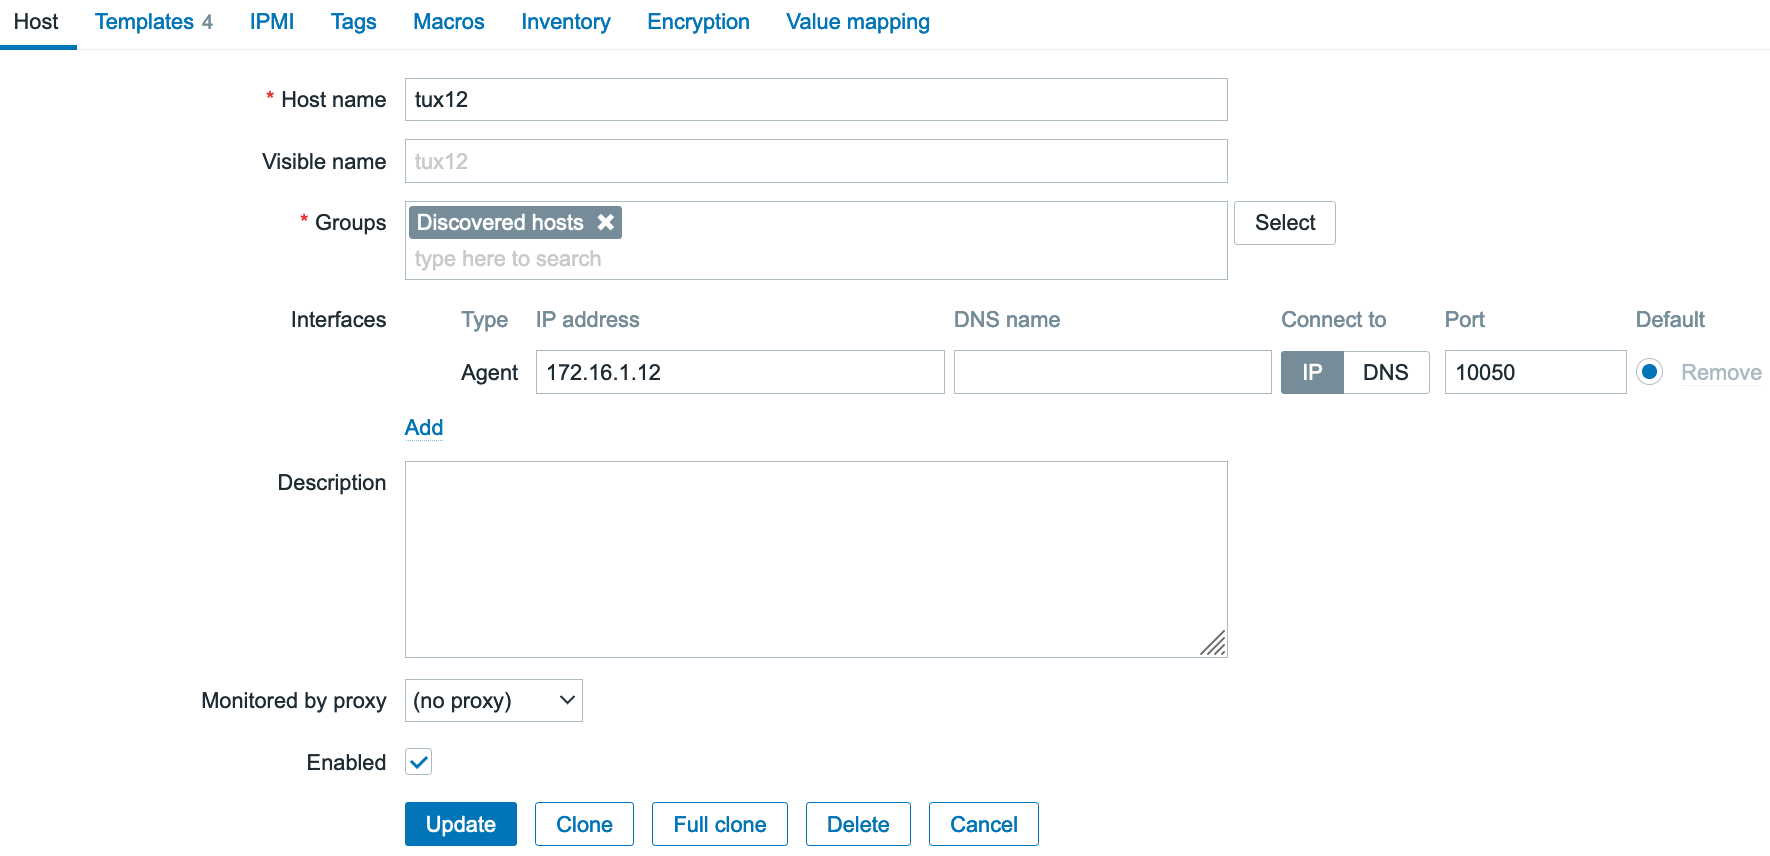
\includegraphics[width=.9\linewidth]{figs/zabbix/tux12_setup_1}
        \caption{Interface do Tux12 - Agent}
        \label{fig:tux12_setup_1}
    \end{subfigure}
    \hfill
    \begin{subfigure}[b]{0.9\textwidth}
        \centering
        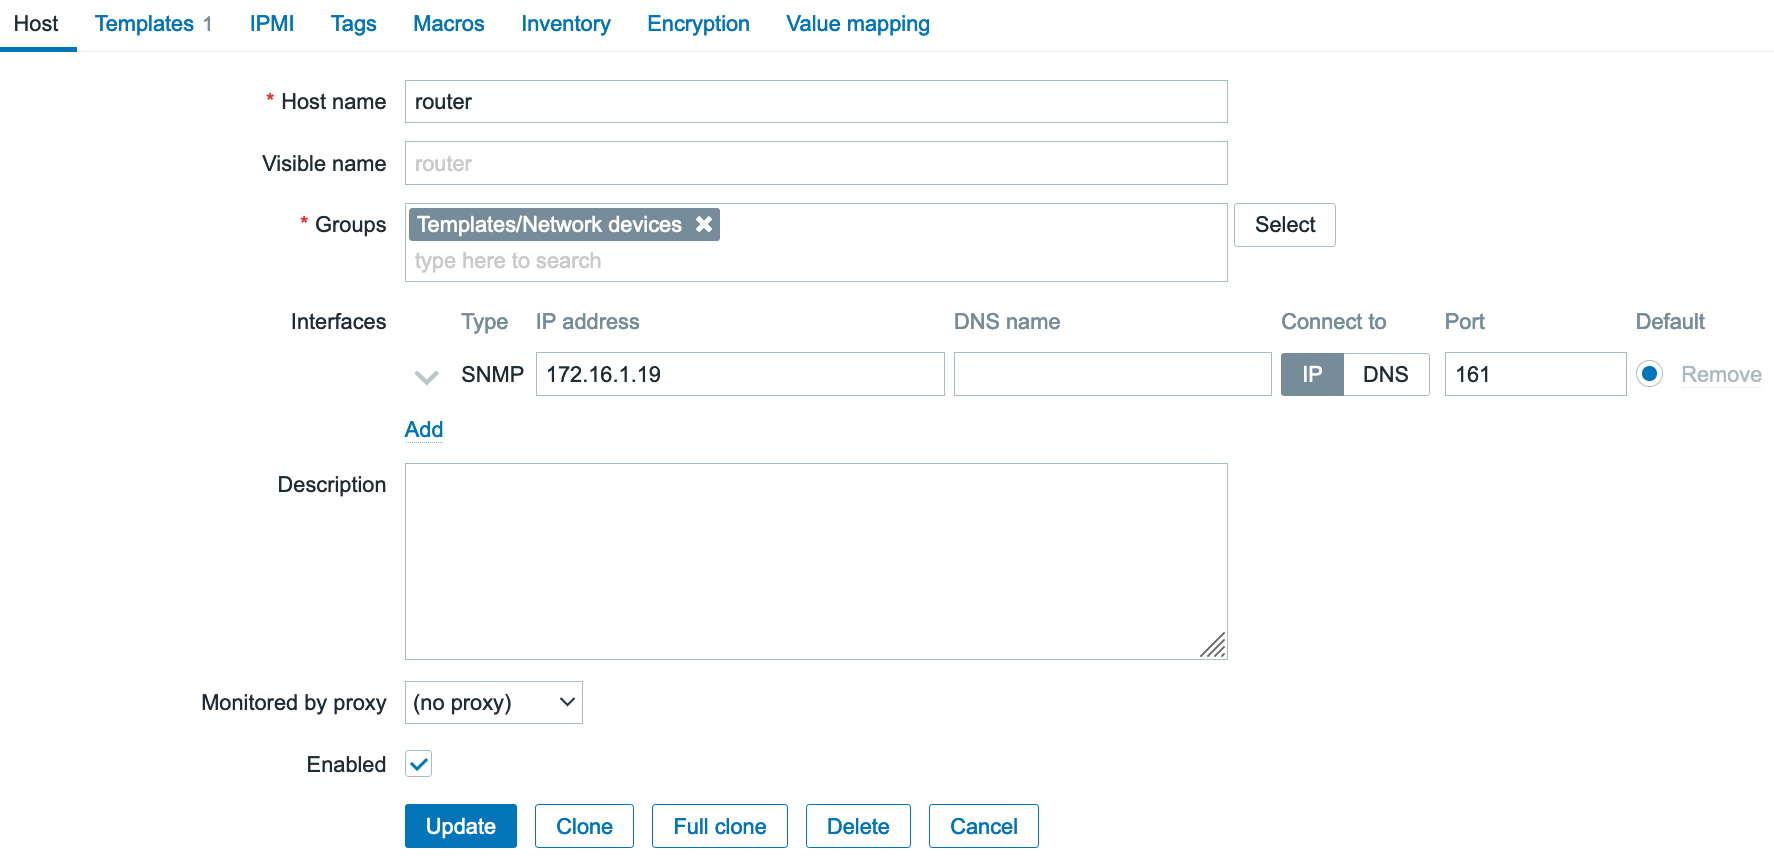
\includegraphics[width=.9\linewidth]{figs/zabbix/router_setup_1}
        \caption{Interface do Router - SNMP}
        \label{fig:router_setup_1}
    \end{subfigure}
    \caption{}
\end{figure}

Após se assegurar a comunicação entre os diferentes sistemas, é iniciada a configuração da monitorização dos diferentes serviços.

\pagebreak

Similarmente ao Nagios, e dependendo do hosts (Agent ou Agentless) e dos serviços nele alojados, os seguintes templates foram adicionados a cada um:

\begin{table}[H]
    \begin{center}
        \begin{tabular}{ || c | c ||}
        \hline
        \textbf{Sistema} & \textbf{Testes}\\ 
        \hline
        Tux12 & \begin{tabular}{@{}c@{}}Template App Zabbix Agent \\ Template App NTP Service \\ Template App FTP Service \\ Template App SMTP Service\end{tabular}\\
        \hline
        Tux14 & \begin{tabular}{@{}c@{}}Template App Zabbix Agent \\ Template App HTTP Service\\ Template App SMTP Service\end{tabular}\\
        \hline
        Router & Template Module Generic SNMPv2\\
        \hline
        Switch & Template Module Generic SNMPv2\\
        \hline
        Tux13 & \begin{tabular}{@{}c@{}}Template App Zabbix Server \\ Template App Zabbix Agent \\ \end{tabular}\\
        \hline
        
        \end{tabular}
    \end{center}    
    \caption{Alocação dos serviços nos computadores}
    \label{tab:template_table}
\end{table}


\begin{figure}[H]
    \centering
    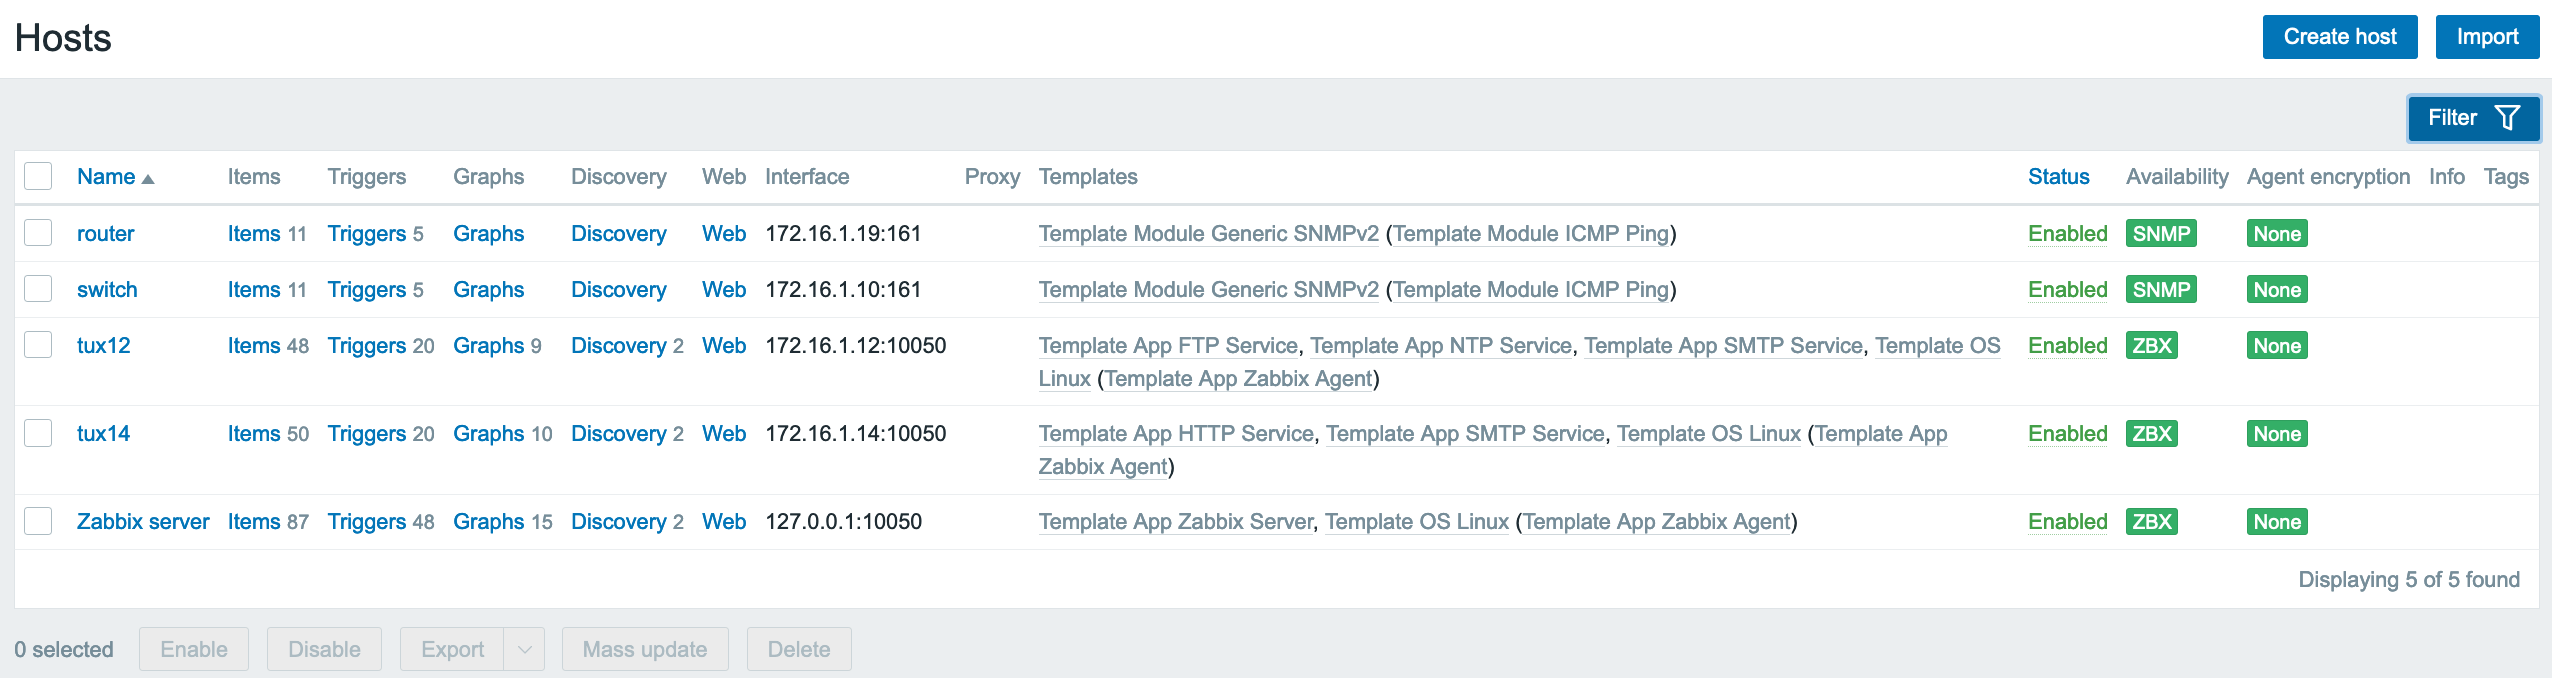
\includegraphics[width=\linewidth]{figs/zabbix/hosts_templates}
    \caption{Templates associados a cada host}
    \label{fig:hosts_templates}
\end{figure}


Como se pode observar, nenhum template associado ao serviço DNS foi adicionado.
De facto, o Zabbix não fornece nenhum template default para esse fim.
Embora seja possível importar templates externos, foi configurado um item e o correspondente trigger manualmente.

\begin{figure}[H]
    \centering
    \begin{subfigure}[b]{0.49\textwidth}
        \centering
        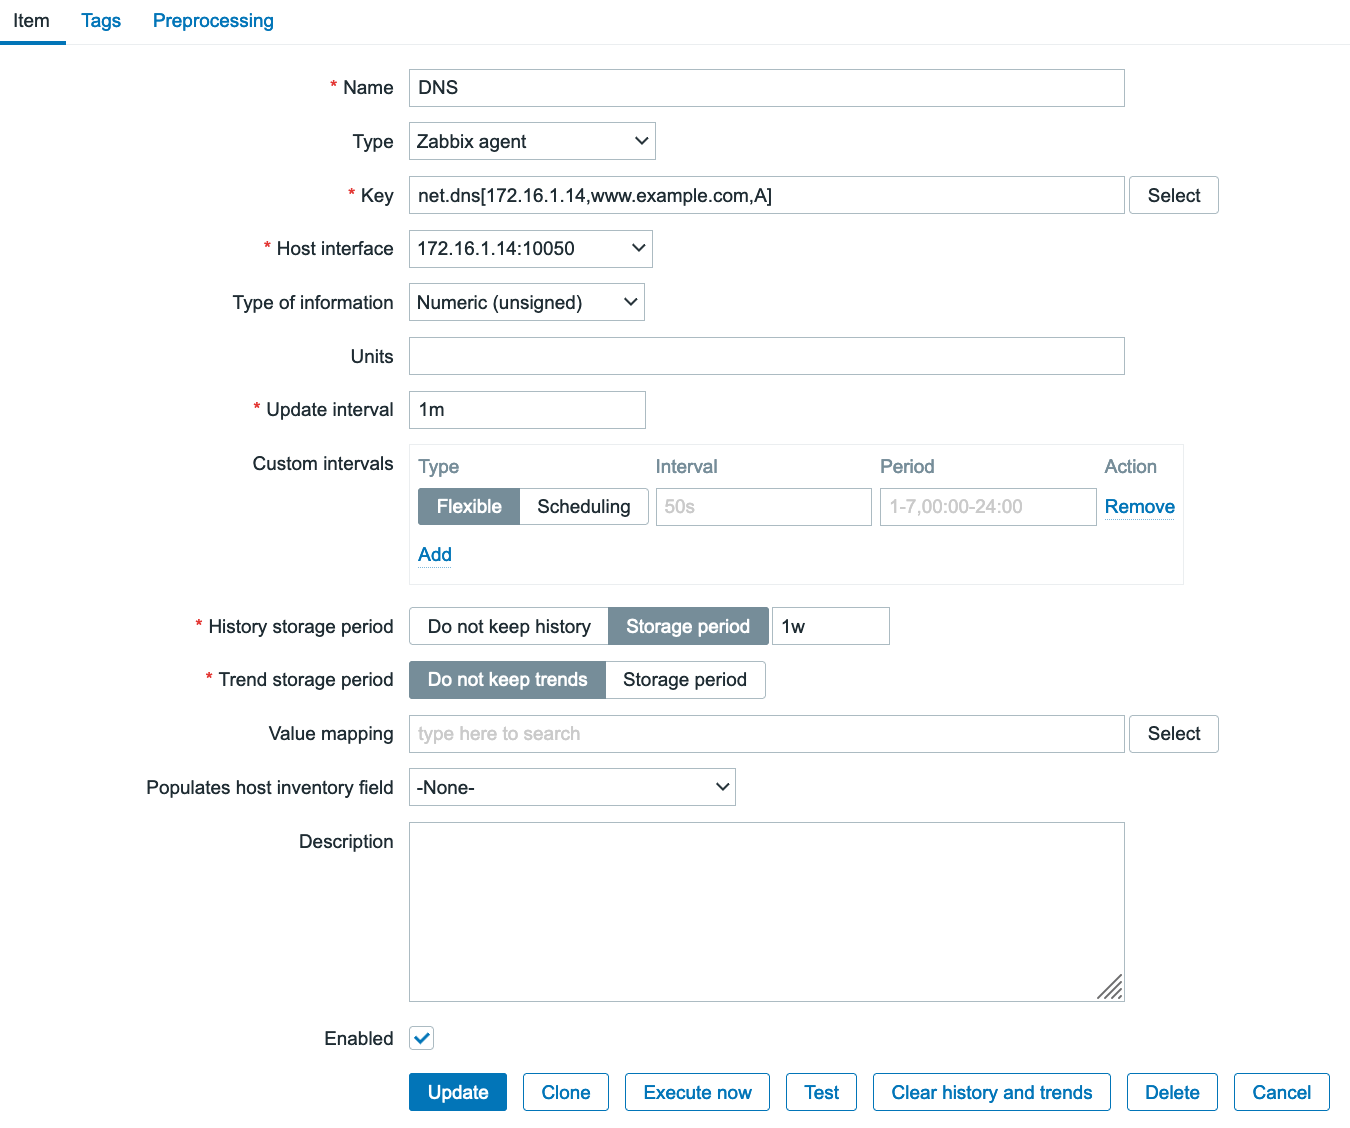
\includegraphics[width=.9\linewidth]{figs/zabbix/dns_item}
        \caption{Item DNS}
        \label{fig:dns_item}
    \end{subfigure}
    \hfill
    \begin{subfigure}[b]{0.49\textwidth}
        \centering
        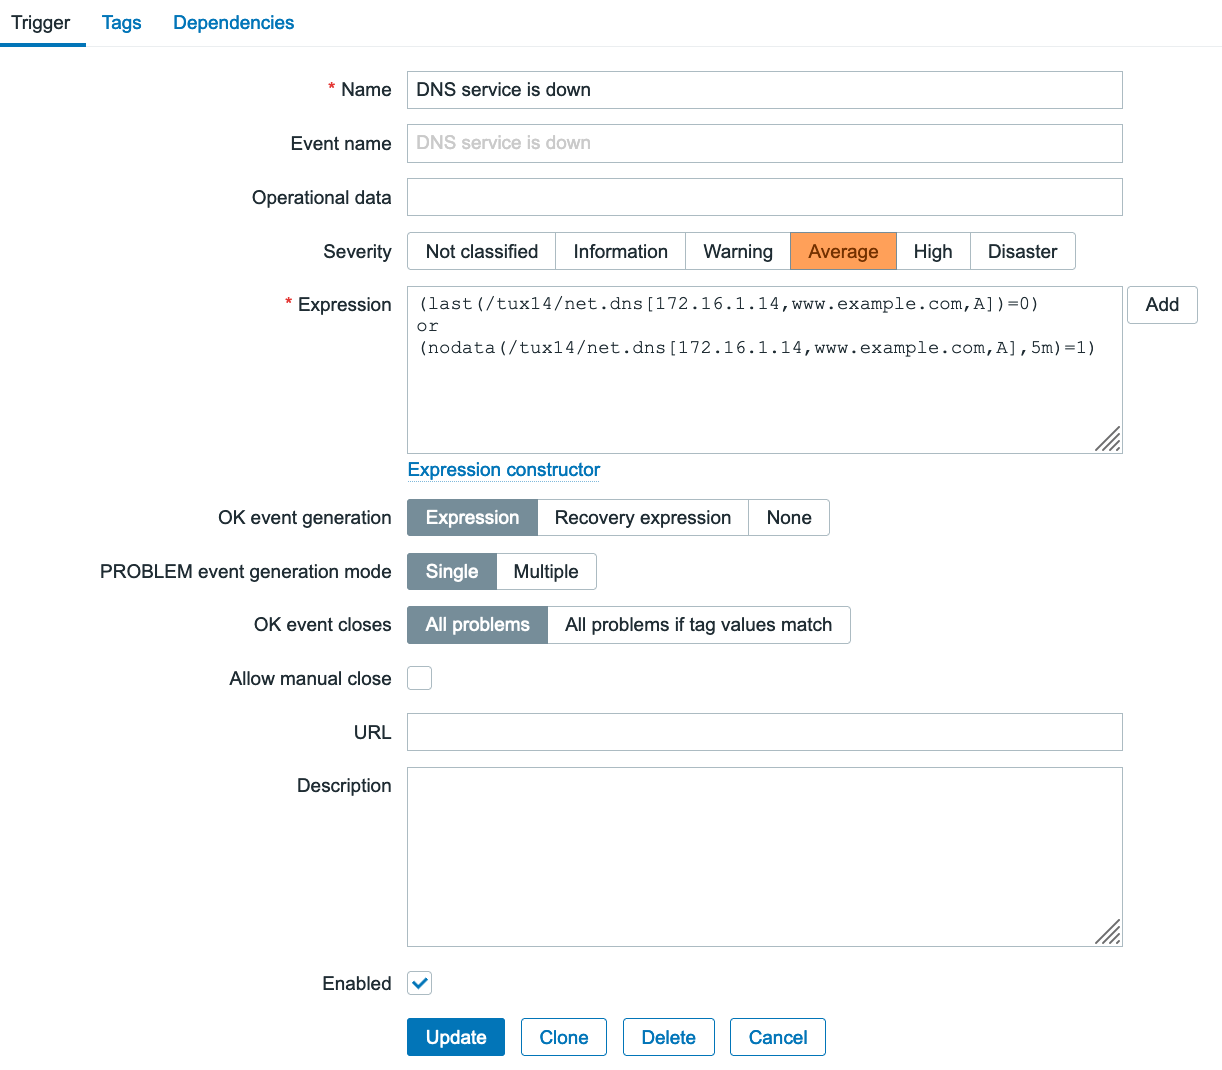
\includegraphics[width=.9\linewidth]{figs/zabbix/dns_trigger}
        \caption{Trigger DNS}
        \label{fig:dns_trigger}
    \end{subfigure}
    \caption{}
\end{figure}

Este teste verifica se a \textit{query} feita ao servidor DNS é respondida. 
Se tal não se verificar, ou se não se obtiver resposta do host de todo, um alerta da gravidade \textit{Average}, igual ao de outros serviços, é criado.

\pagebreak

\section{Resultados}


\begin{figure}[H]
    \centering
    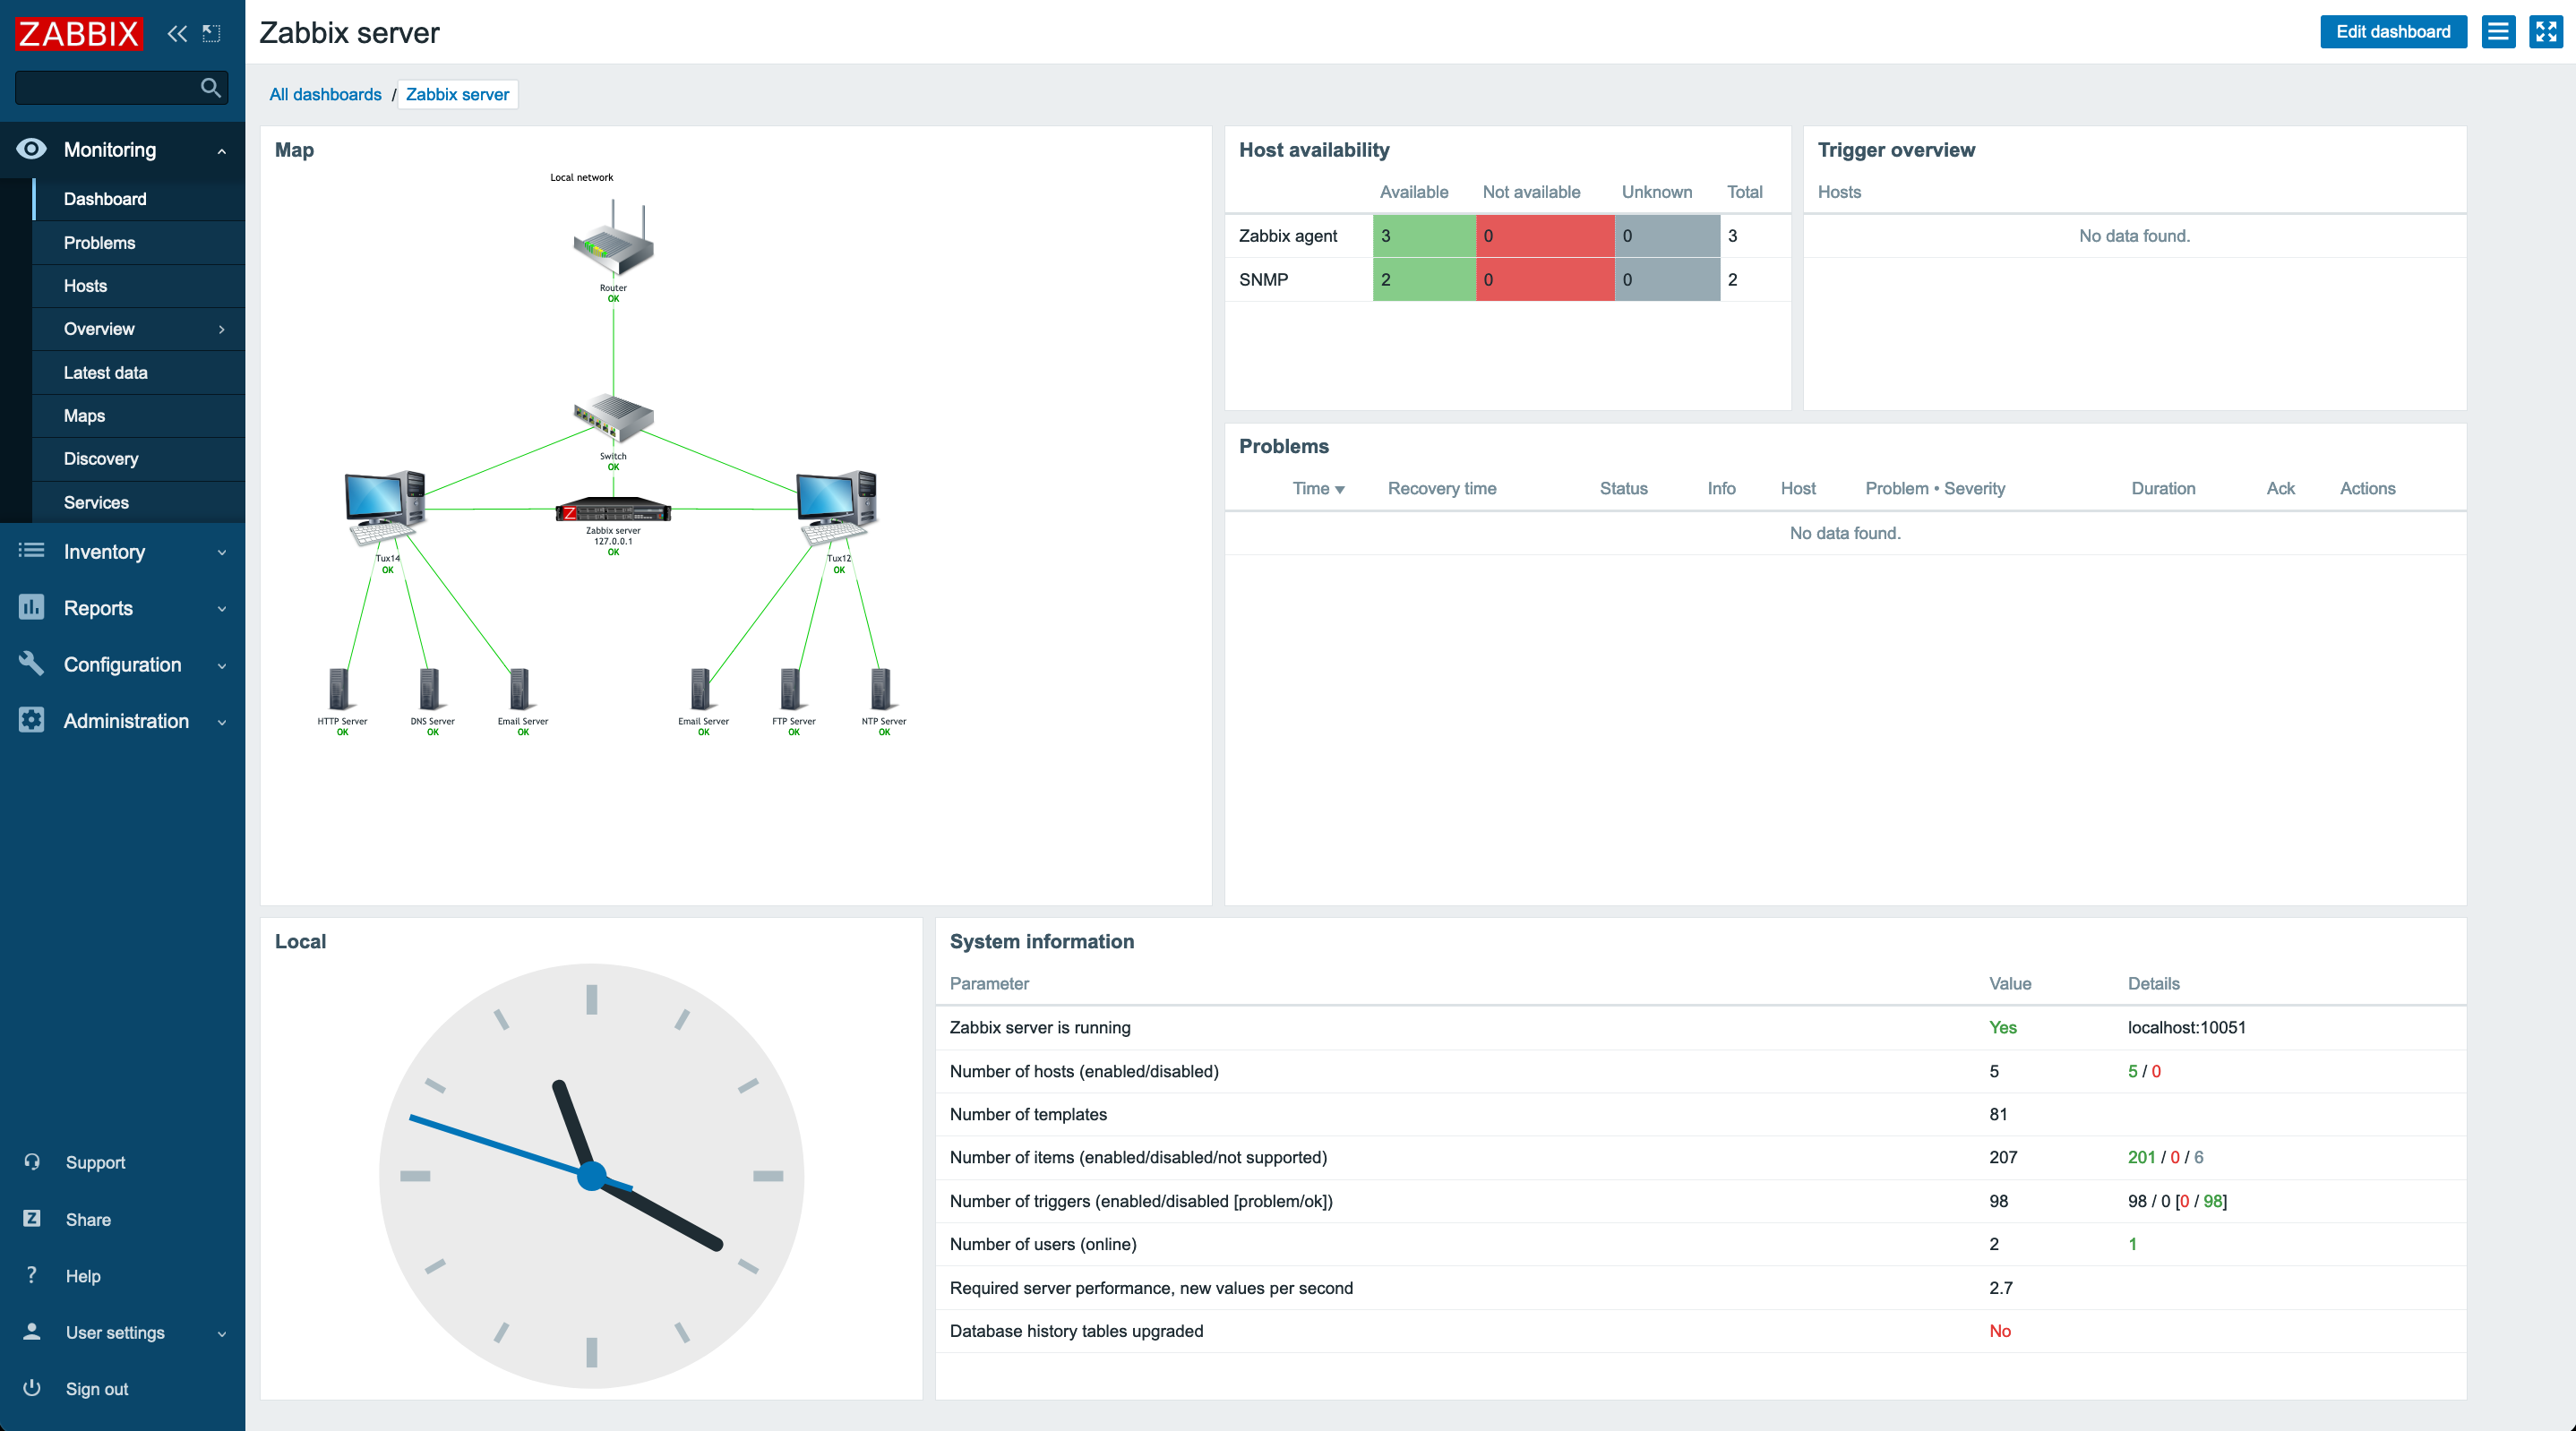
\includegraphics[width=\linewidth]{figs/zabbix/zabbix_dashboard}
    \caption{Dashboard principal}
    \label{fig:zabbix_dashboard}
\end{figure}

Uma das principais vantagens do Zabbix é o seu grau de customização, nomeadamente as \textbf{Dashboards}.
Esta dashboard foi criada por nós, onde a informação mais relevante é apresentada:
\begin{itemize}
    \item Hosts Availability: Quantos hosts então \textit{up/down}.
    \item Trigger Overview: Quais foram os triggers que foram despoletados.
    \item Problems: Quais os problemas do rede.
    \item System Information: Compilação geral da configuração do sistema e status da rede.
    \item Local: Hora local definida no servidor, neste caso \textit{Europe/Lisbon}.
    \item MAP: Interface que permite de uma forma visual verificar o status de serviços e hosts.
    Este mapa foi desenhado por nós para apresentar todos os hosts e os serviços neles alojados.
    É possívelmente a componente mais importante pois apresenta pragmaticamente e de forma simples toda a informação relevante neste trabalho.
\end{itemize}

Existem muitas outras interfaces com compilação de informação do sistema.
É também possível ver a evolução do status de alguns parâmetros graficamente ou o histórico de outputs.

\pagebreak

\section{Teste de falhas}

Os testes de falhas no Nagios e no Zabbix foram executados ao mesmo tempo, pelo que o método é o mesmo:
\begin{center}
    Tux12 \\
    \verb|systemctl stop vsftpd - Falha do servidor FTP| \\
    \verb|systemctl stop postfix - Falha do servidor Email| \\

    \vspace{1cm}
    Tux14 \\
    \verb|systemctl stop bind9 - Falha do servidor DNS| \\
    \verb|systemctl stop apache2 - Falha do servidor HTTP|
\end{center}

Após algum tempo de atualização de informação, o output da interface do Zabbix foi o seguinte:

\begin{figure}[H]
    \centering
    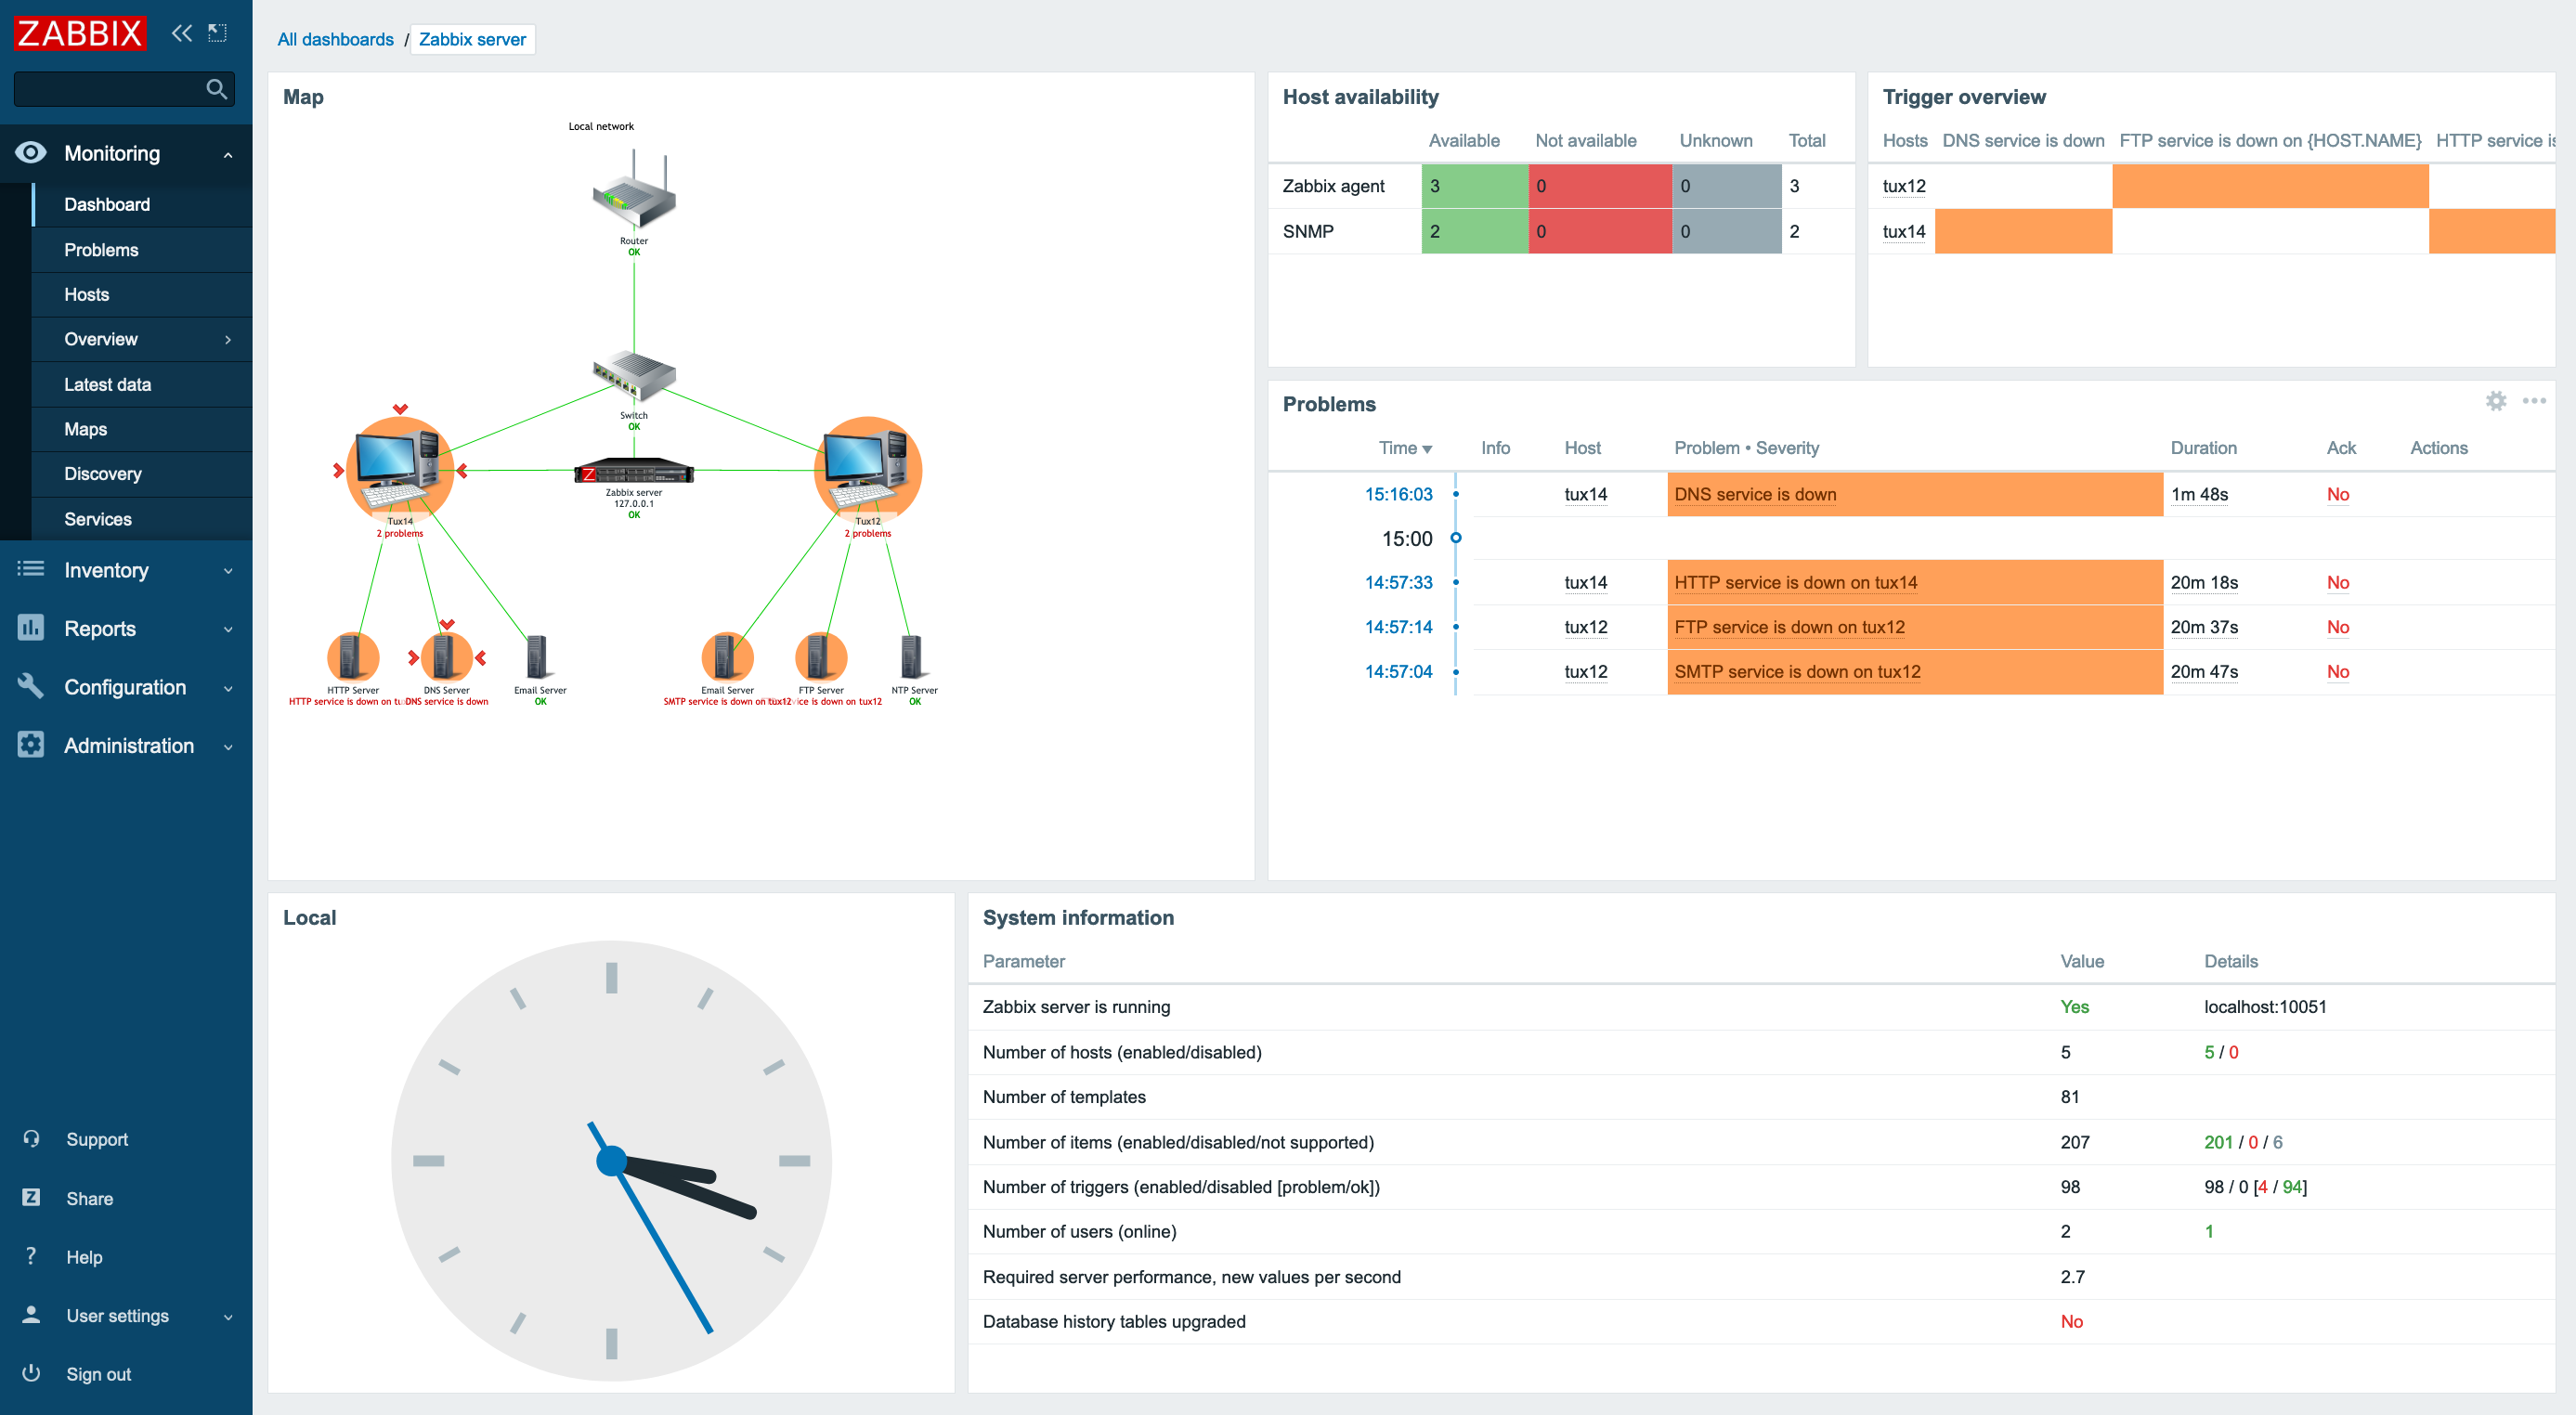
\includegraphics[width=\linewidth]{figs/zabbix/zabbix_errors}
    \caption{Falha de serviços}
    \label{fig:zabbix_errors}
\end{figure}

O Zabbix apresenta na tab \textit{Problems} quais são os problemas encontrados, neste caso os serviços down, assim como o \textit{timestamp} associado ao evento.
É possível também observar quais foram os triggers despoletados, e em que hosts ocorreram.
Por fim, de uma forma mais visual, os hosts onde há problemas são destacados com a cor do problema mais grave, neste caso de severidade \textit{Average} que corresponde ao laranja.

Consequentemente, simulou-se a falha do Tux14, obtendo-se os seguintes resultados:

\begin{figure}[H]
    \centering
    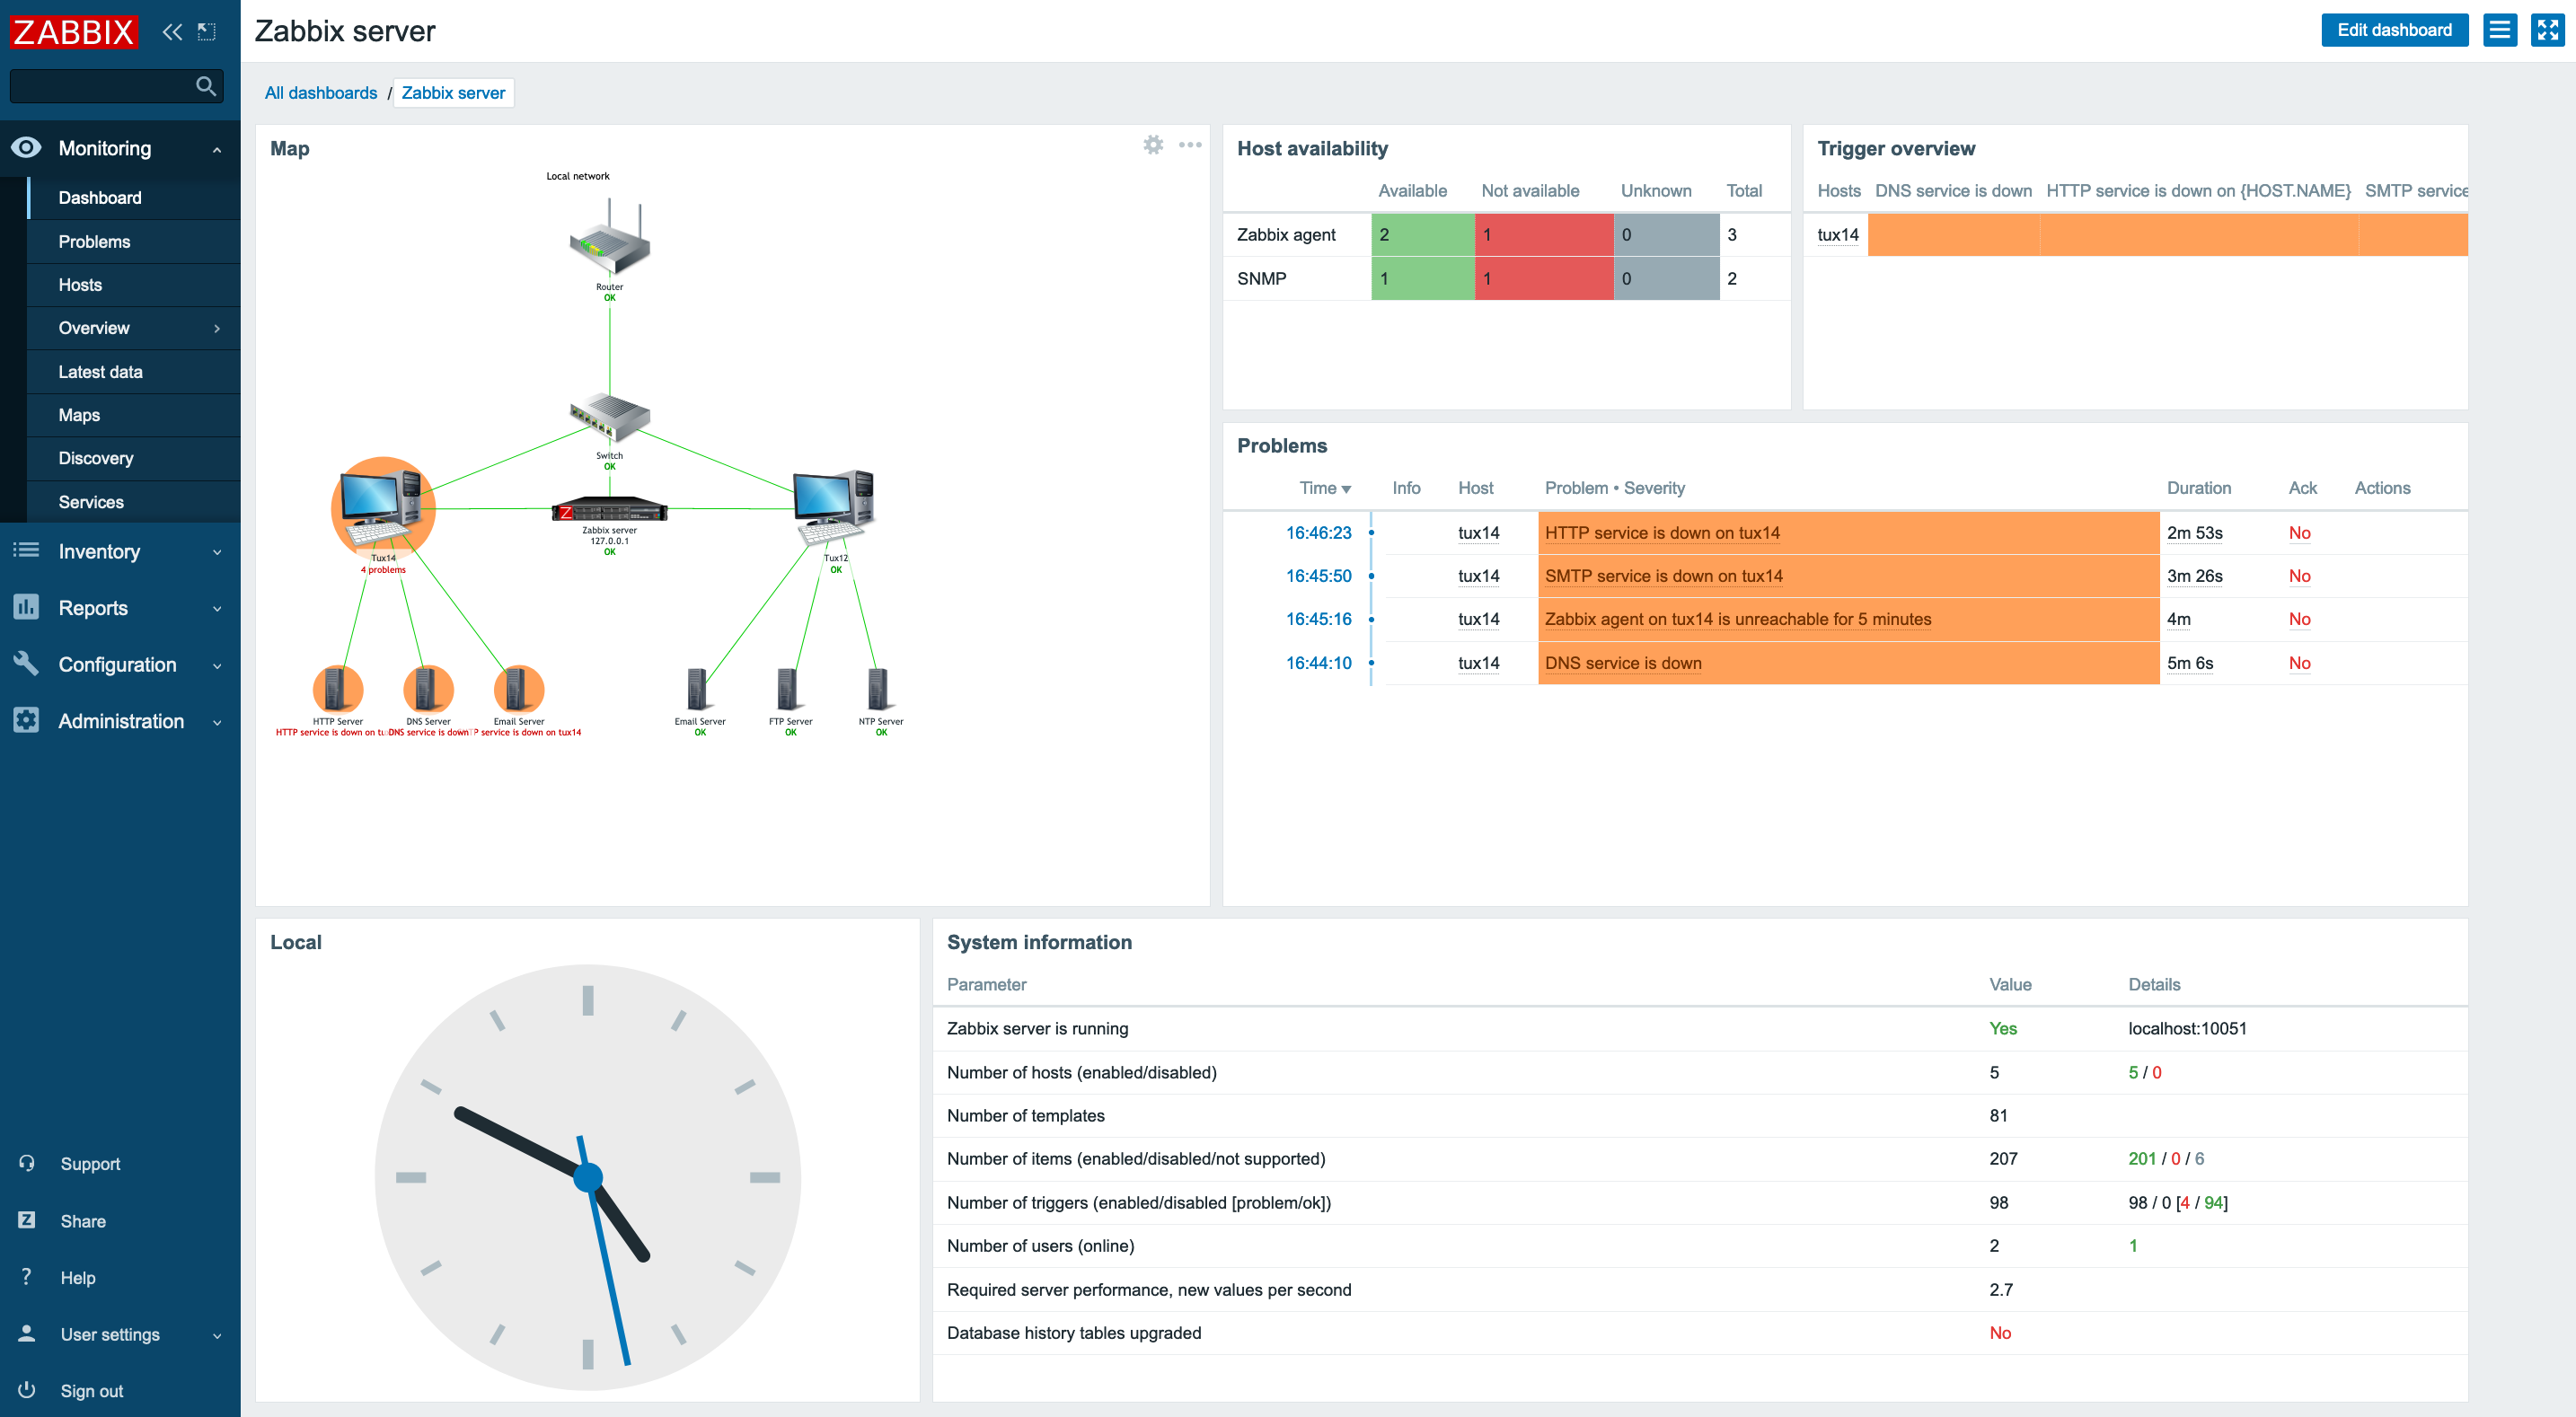
\includegraphics[width=\linewidth]{figs/zabbix/zabbix_tux14_down}
    \caption{Falha do Tux14}
    \label{fig:zabbix_tux14_down}
\end{figure}

É possível observar que o Zabbix indica que se perdeu contacto com o agente no Tux14.
Desse modo, na tab \textit{Host availability}, já se observa que um host está down.
Os serviços alojados no host que falhou também falharam todos, como se pode ver quer no mapa, quer na tab \textit{Problems}.

Sabendo que o host foi desligado às 16:40, o Zabbix demorou 4 minutos a detetar a falhar no sistema, sendo que o estado serviços foi atualizado pouco depois.
É de salientar que a frequência de teste pode ser alterado igualmente na configuração do Zabbix.